\section{Introduction}
%
%
\begin{frame}
  In this talk we will discuss the error incurred when generalizing a learning
  model to unseen data.
\end{frame}
%
%
\begin{frame}
  We will see that this error comes from three distinct sources:
\end{frame}
%
%
\begin{frame}
  First is the error that results from the inherent randomness in the quantity
  being modeled.

  \begin{figure}
    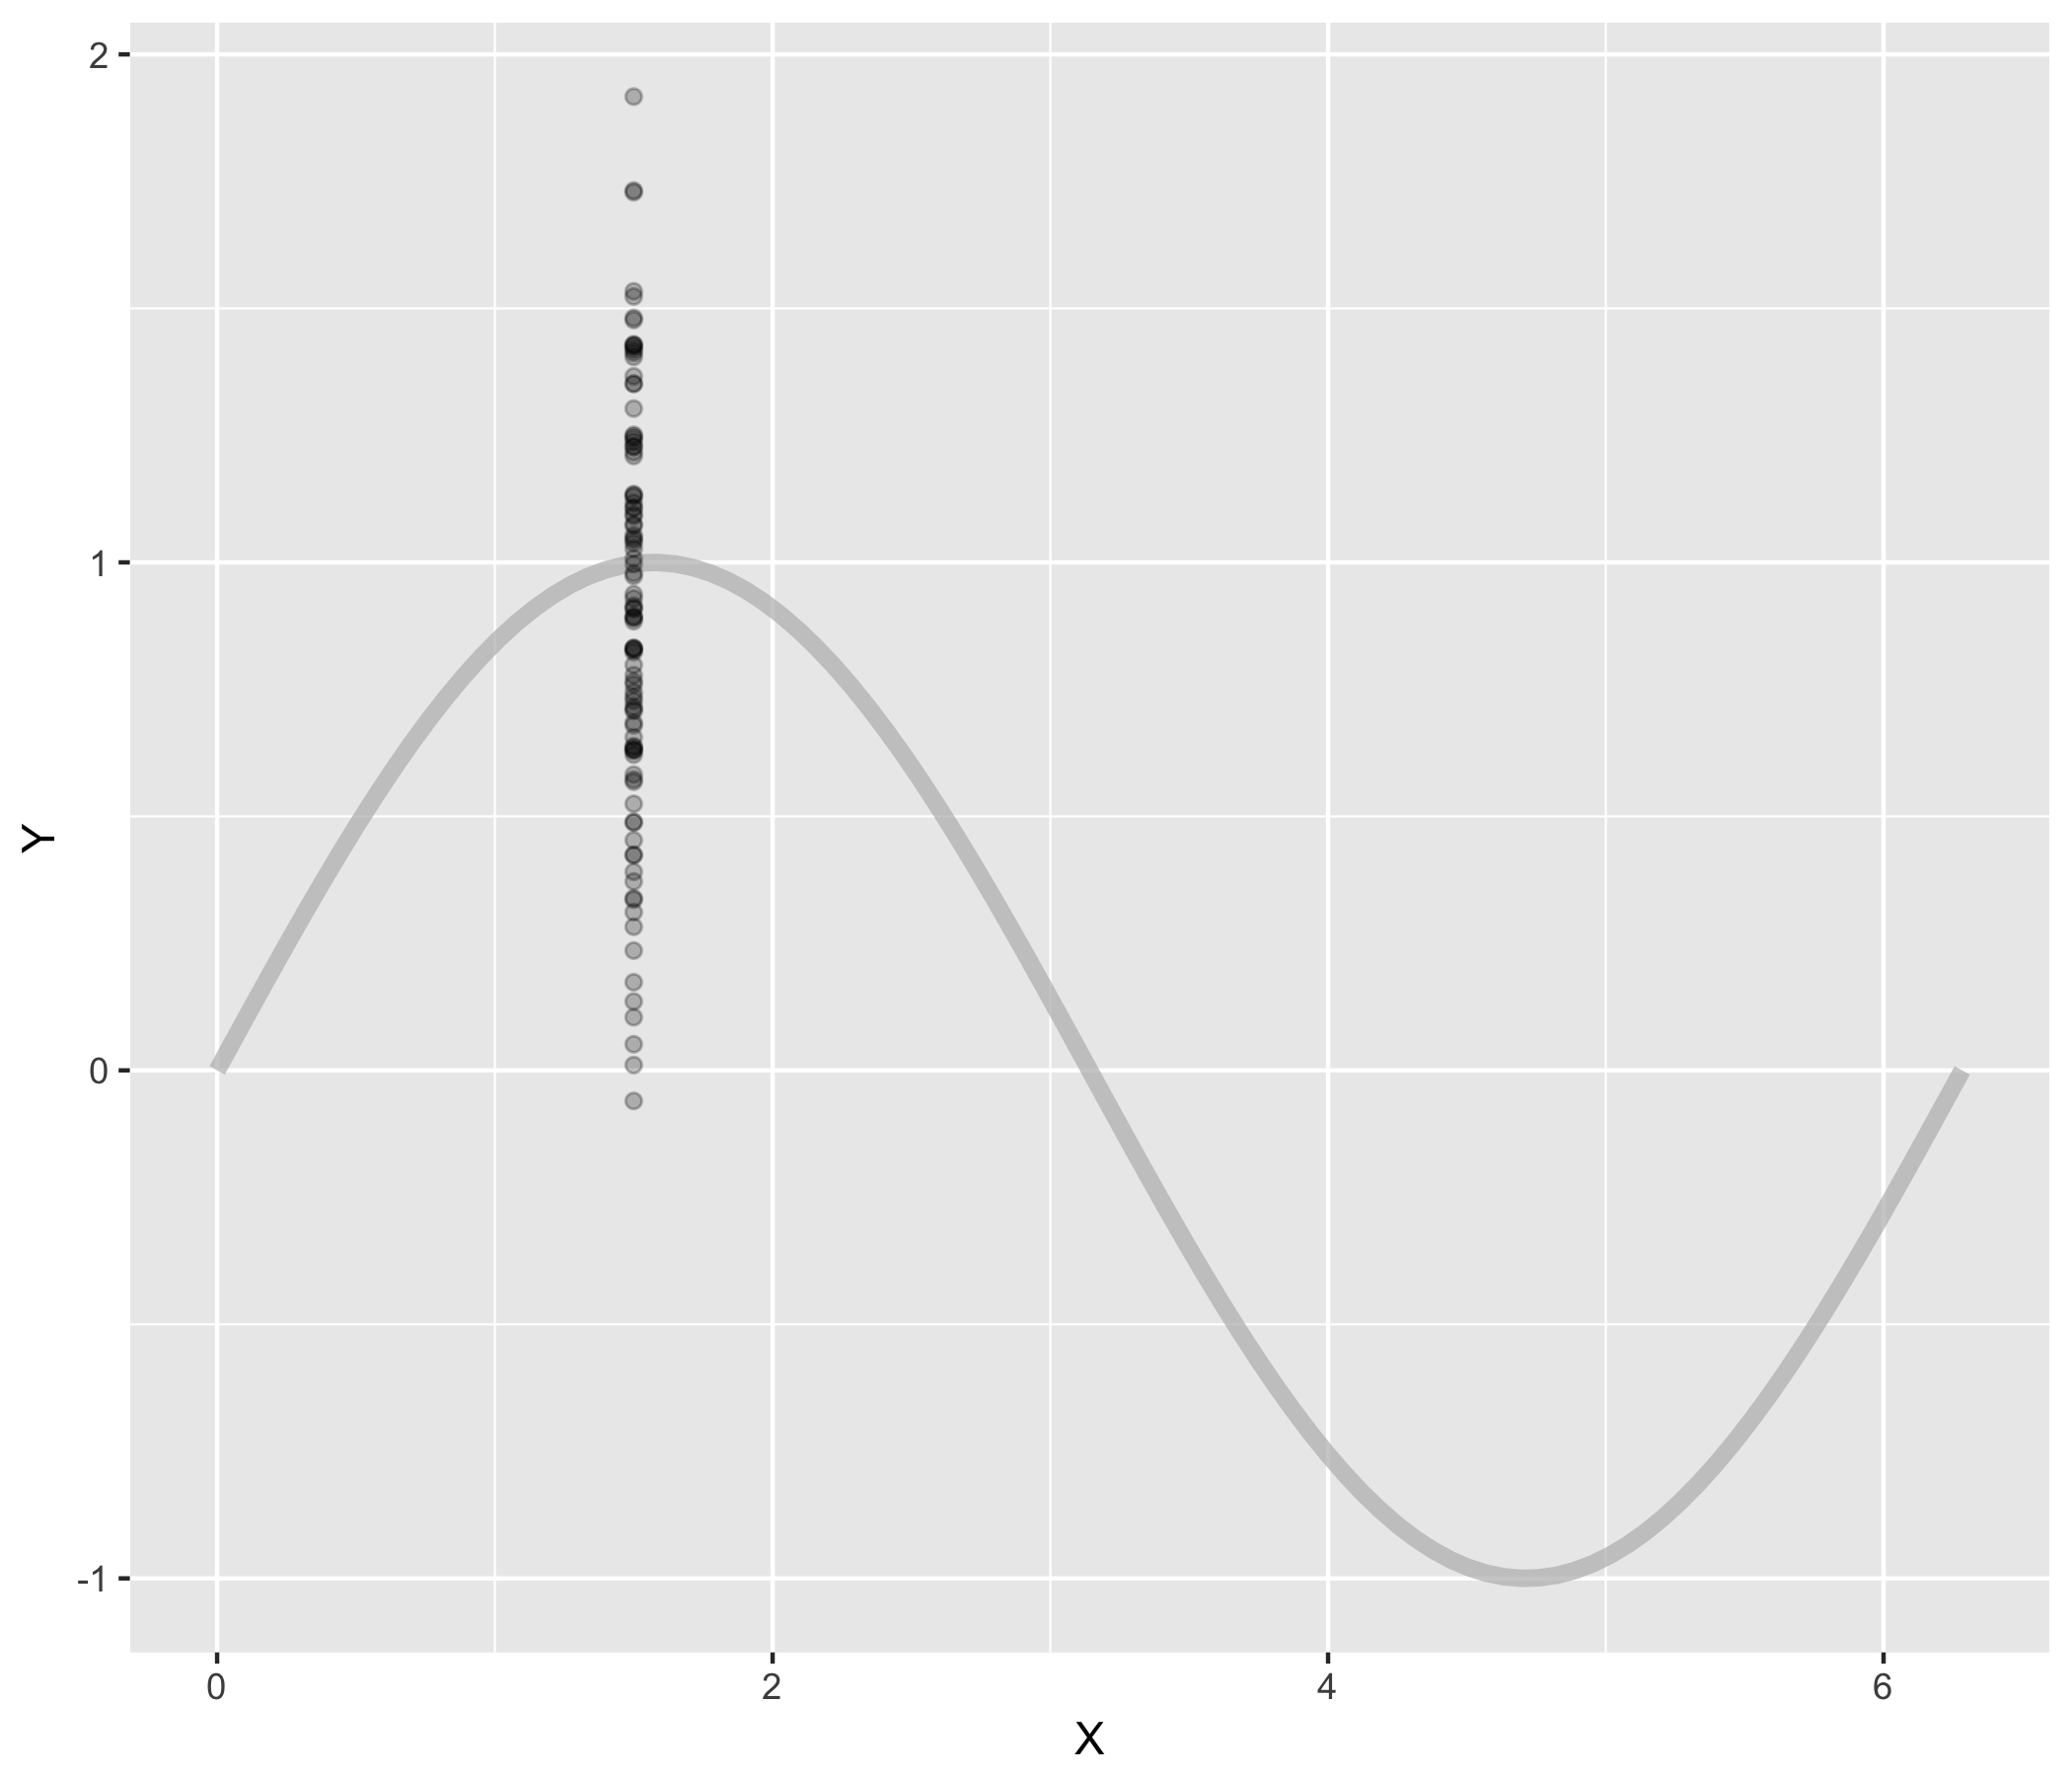
\includegraphics[scale=0.09]{irreducible_error}
  \end{figure}

  This is called the \textbf{irreducible error}
\end{frame}
%
%
\begin{frame}
  Second is the error incurred from misspecification of the model, resulting in
  an inability of the model to adapt to the target.

  \begin{figure}
    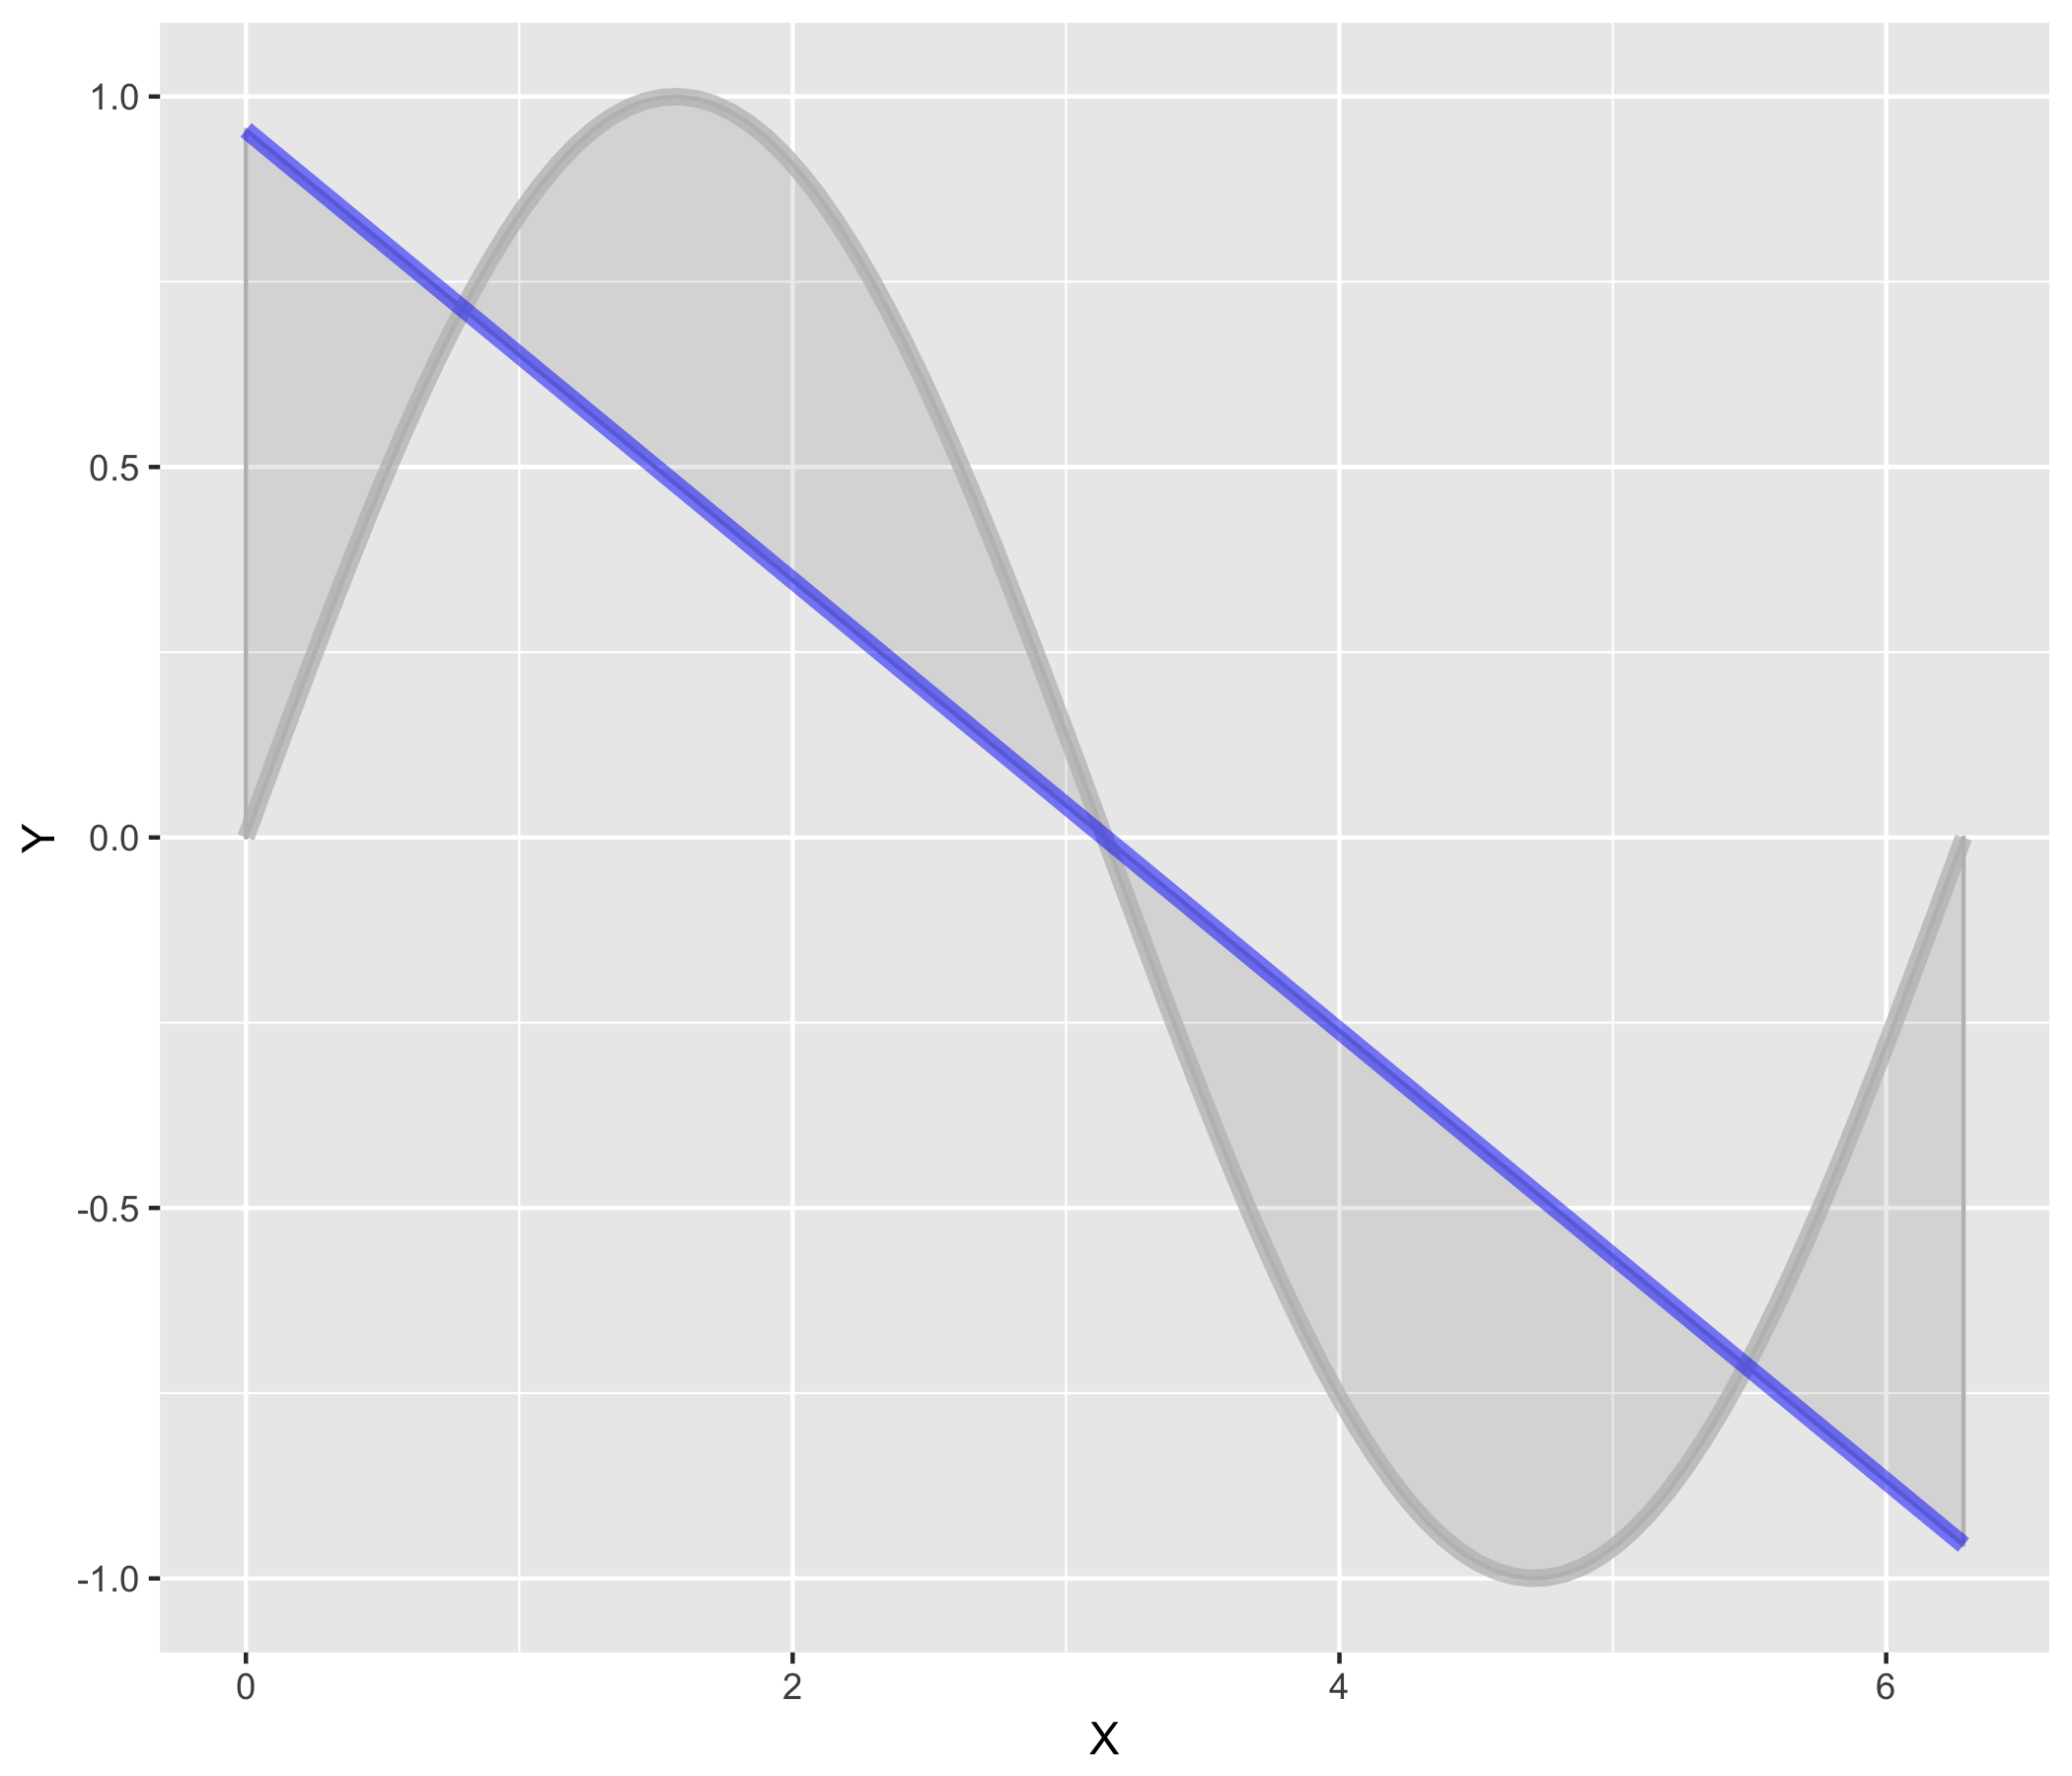
\includegraphics[scale=0.09]{model_bias}
  \end{figure}

  This is called the \textbf{model bias}.
\end{frame}
%
%
\begin{frame}
  Finally is the error incurred because our training data is not fully
  informative of random process at work, causing the model to deviate from the
  ideal fit.

  \begin{figure}
    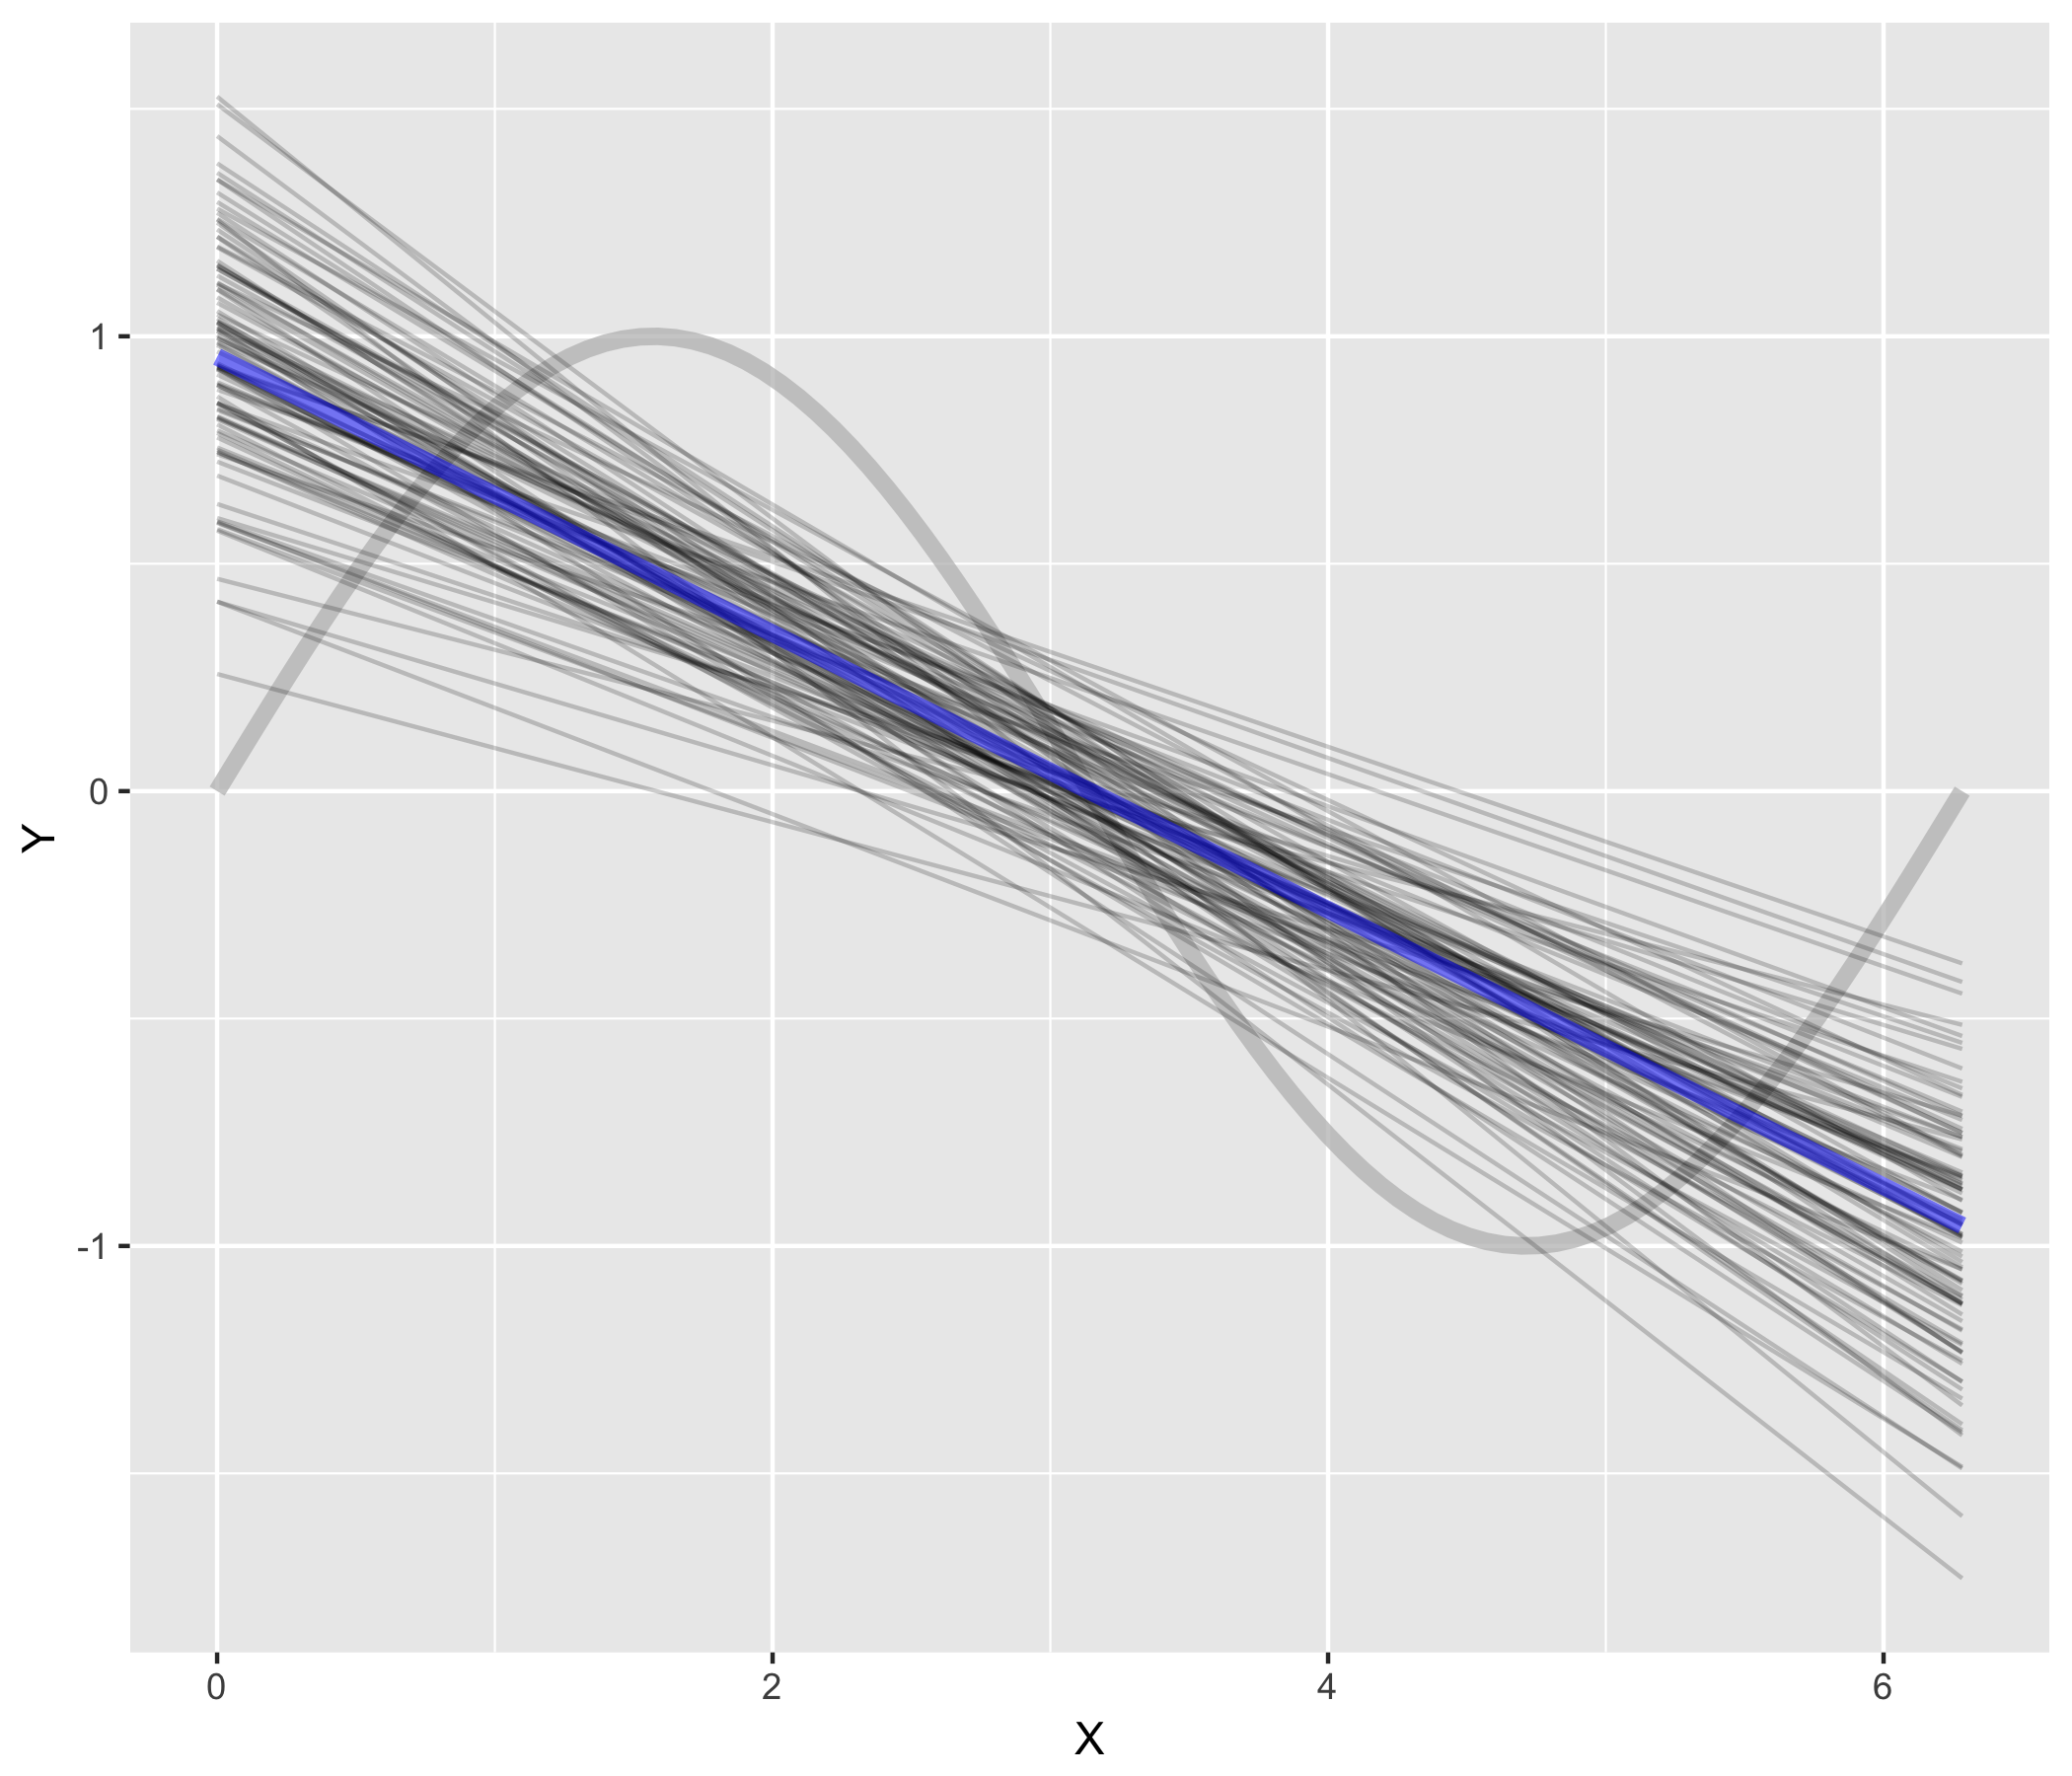
\includegraphics[scale=0.09]{model_variance}
  \end{figure}

  This is called the \textbf{model variance}.
\end{frame}
